
%%% ====================================================================
%%% Exemplo de construção da folha de aprovação. Depois da
%%% apresentação do trabalho, quando a folha de apresentação real
%%% tiver sido assinada pela banca, a folha real deve ser digitalizada
%%% e o ambiente abaixo deve ser substituído por:
%%% \includepdf{folhadeaprovacao_final.pdf}
\begin{folhadeaprovacao}
  \begin{center}
    {\ABNTEXchapterfont\MakeTextUppercase{\imprimirautor}}\\
    \begin{center}
      \ABNTEXchapterfont\MakeTextUppercase{\imprimirtitulo}\\
    \end{center}
    \hspace{.45\textwidth}
    \begin{minipage}{.5\textwidth}
      {\footnotesize{\imprimirpreambulo}}\\
    \end{minipage}%
  \end{center}
  \vspace{-1cm}%
  \begin{center}
    Aprovado em 26 de Novembro de 2019.\\[15mm]
    \textbf{COMISSÃO EXAMINADORA}\\[5mm]
    \begin{figure}[H]
    	\centering % para centralizarmos a figura
    	\advance\rightskip-1.3cm
    	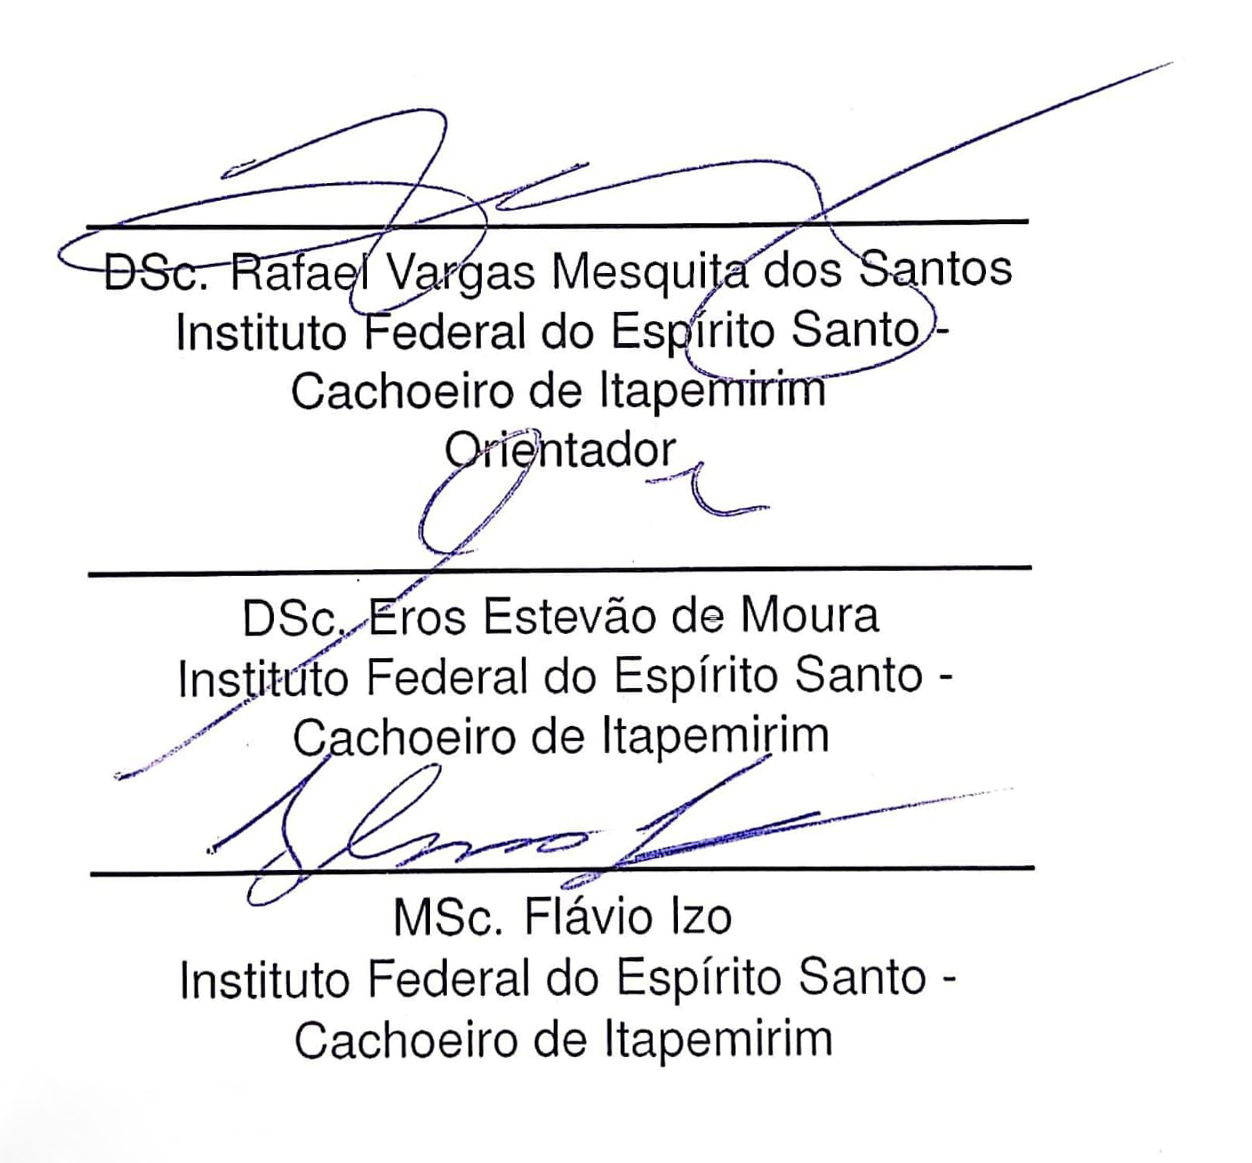
\includegraphics[width=12cm]{resources/aprovacao.png} % leia abaixo
    \end{figure}
    % \assinatura{\imprimirorientador \\
    %   Instituto Federal do Espírito Santo - Cachoeiro de Itapemirim \\ Orientador}\vspace{-1cm}
    % \assinatura{DSc. Eros Estevão de Moura \\
    %   Instituto Federal do Espírito Santo - Cachoeiro de Itapemirim}\vspace{-1cm}
    % \assinatura{MSc. Flávio Izo\\
    %   Instituto Federal do Espírito Santo - Cachoeiro de Itapemirim}\vspace{-1cm}
  \end{center}
  
\end{folhadeaprovacao}